%%%%%%%%%%%%%%%%%%%%%%%%%%%%%%%%%%%%
% Don't touch these options
%%%%%%%%%%%%%%%%%%%%%%%%%%%%%%%%%%%%


\documentclass[english, 11pt]{article}\usepackage[]{graphicx}\usepackage[]{color}
%% maxwidth is the original width if it is less than linewidth
%% otherwise use linewidth (to make sure the graphics do not exceed the margin)
\makeatletter
\def\maxwidth{ %
  \ifdim\Gin@nat@width>\linewidth
    \linewidth
  \else
    \Gin@nat@width
  \fi
}
\makeatother

\definecolor{fgcolor}{rgb}{0.345, 0.345, 0.345}
\newcommand{\hlnum}[1]{\textcolor[rgb]{0.686,0.059,0.569}{#1}}%
\newcommand{\hlstr}[1]{\textcolor[rgb]{0.192,0.494,0.8}{#1}}%
\newcommand{\hlcom}[1]{\textcolor[rgb]{0.678,0.584,0.686}{\textit{#1}}}%
\newcommand{\hlopt}[1]{\textcolor[rgb]{0,0,0}{#1}}%
\newcommand{\hlstd}[1]{\textcolor[rgb]{0.345,0.345,0.345}{#1}}%
\newcommand{\hlkwa}[1]{\textcolor[rgb]{0.161,0.373,0.58}{\textbf{#1}}}%
\newcommand{\hlkwb}[1]{\textcolor[rgb]{0.69,0.353,0.396}{#1}}%
\newcommand{\hlkwc}[1]{\textcolor[rgb]{0.333,0.667,0.333}{#1}}%
\newcommand{\hlkwd}[1]{\textcolor[rgb]{0.737,0.353,0.396}{\textbf{#1}}}%
\let\hlipl\hlkwb

\usepackage{framed}
\makeatletter
\newenvironment{kframe}{%
 \def\at@end@of@kframe{}%
 \ifinner\ifhmode%
  \def\at@end@of@kframe{\end{minipage}}%
  \begin{minipage}{\columnwidth}%
 \fi\fi%
 \def\FrameCommand##1{\hskip\@totalleftmargin \hskip-\fboxsep
 \colorbox{shadecolor}{##1}\hskip-\fboxsep
     % There is no \\@totalrightmargin, so:
     \hskip-\linewidth \hskip-\@totalleftmargin \hskip\columnwidth}%
 \MakeFramed {\advance\hsize-\width
   \@totalleftmargin\z@ \linewidth\hsize
   \@setminipage}}%
 {\par\unskip\endMakeFramed%
 \at@end@of@kframe}
\makeatother

\definecolor{shadecolor}{rgb}{.97, .97, .97}
\definecolor{messagecolor}{rgb}{0, 0, 0}
\definecolor{warningcolor}{rgb}{1, 0, 1}
\definecolor{errorcolor}{rgb}{1, 0, 0}
\newenvironment{knitrout}{}{} % an empty environment to be redefined in TeX

\usepackage{alltt}
\usepackage[T1]{fontenc}
\usepackage[latin9]{inputenc}
\usepackage{geometry}
\geometry{verbose,tmargin=2.5cm,bmargin=2.5cm,lmargin=2.5cm,rmargin=2.5cm}
\usepackage{float}
\usepackage{graphicx}
\usepackage{babel}
\usepackage{hyperref}
\usepackage{bm}
\IfFileExists{upquote.sty}{\usepackage{upquote}}{}
\begin{document}

%%%%%%%%%%%%%%%%%%%%%%%%%%%%%%%%%%%%
% Title Page
%%%%%%%%%%%%%%%%%%%%%%%%%%%%%%%%%%%%
\title{Unsupervised Learning of Cellular Development Time}


\author{Caleb Lareau}


\date{11 May 2017}
\maketitle
\begin{abstract}
\noindent Recent advances in microfluidic technologies have enabled an unprecedented characterization of epigenomic and transcriptomic profiles of single cells. Though the dimension of the single cell feature space often exceeds 20,000, a commonly desired yet unobserved variable associated with cellular development time must be estimated using computational methods. Herein, I motivate the approximation of this latent dimension termed \textit{pseudotime} and contextualize its inference as an application of unsupervised learning. Moreover, I present the statistical basis of both linear (principal component analysis; PCA) and non-linear (Gaussian process latent variable modeling; GPLVM) dimension reduction from a probabilistic perspective. To evaluate the performance of the methods of unsupervised learning in this context, I examine the inferred pseudotime against the true developmental ordering of murine embryonic stem cell maturation. 

\newpage{}
\end{abstract}

%%%%%%%%%%%%%%%%%%%%%%%%%%%%%%%%%%%%
% End Title Page
%%%%%%%%%%%%%%%%%%%%%%%%%%%%%%%%%%%%




%%%%%%%%%%%%%%%%%%%%%%%%%%%%%%%%%%%%
\section{Introduction}

A fundamental question in developmental biology is how organisms such as humans and mice that originate as single zygotes mature into complex entities composed of trillions of cells in adulthood. Moreover, identifying the longitudinal genetic and epigenetic factors that control stages of development is critical for understanding disease presentation and manifestation.  Recent technological advances have enabled a high-throughput characterization of single cells, providing a formidable means of identifying factors critical in complex organism development and disease. In particular, the breakthroughs in microfluidic capture and sequencing of RNA from single cells (scRNA-Seq) has incited the development of a ``Human Cell Atlas,'' which expects to profile an estimated 35 trillion cells over the next decade from various stages of human development. \cite{HCA} 
\newline  \newline 
\noindent With this unprecendented source of human cellular data, robust statistical and computational frameworks are needed to extract meaningful structure from the Human Cell Atlas and similar single cell profiles to answer these fundamental questions in developmental biology. In particular, low-dimension latent features like cell-cycle stage and developmental time are often desired to be inferred from a higher dimension feature set (\textit{i.e.} $> 20,000$ gene expression values per cell). As these latent characteristics are almost always unobserved from single cell capture technologies, inference of unobserved features motivate the use of unsupervised learning approaches to approximate latent variables in high-dimensional data. Here, I examine the utility and statistical framework for unsupervised learning through a probablistic lense. 


\subsection{Pseudotime ordering of single cells}

Though the technical advances in profiling single cell transcriptomes has become markedly higher-throughput over the past decade, vital characteristics that define a cell's phenotype is often unprofiled through these techniques. \textbf{Figure 1} provides a graphical overview of a typical experimental design, capture process, and analysis framework for single cell data where a latent variable (color gradient/development time) is left unobserved and must be approximated algorithmically. Aside from specific exceptional experimental settings, both the cell cycle and developmental time of a given cell is left unprofiled though these variables are often of distinct interest to investigators. For example, a computational annotation of developmental time across myeloid differentiation enabled the establishment a ``stemness'' program in acute myeloid leukemia (AML), which was shown to be significantly associated with patient surivival and relapse-free survival. \cite{corces2016lineage} Other applications of these methdologies have been used to infer novel cell types in blood \cite{buenrostro2017single} and the genetic markers that distinguish these cellular processes. Consequently, the availability of scRNA-Seq data coupled with methods of pseudotime inference provide a mechanism for investigating outstanding questions in disease, developmental, and regulatory biology.  \newline \newline
\noindent As shown in \textbf{Figure 1C}, statistical methods are needed to approximate the unobserved latent feature of the data. As the observed features (genes) reflect variation in the unobserved variables, $>15$ computational approaches (recently reviewed in \cite{cannoodt2016computational}) have been developed for inferring the color gradient via methods of unsupervised learning. While many of the proposed approaches perform fairly well in estimating developmental time, few provide uncertainty in the calculations of per-cell pseudotime. As insights from this analysis framework may have clinical \cite{corces2016lineage} implications, reliable methods should seemingly quantify uncertainty in the estimation of pseudotime. As such, I will examine \textbf{probablistic} unsupervised learning techniques and their efficacy in estimation of pseudotime for cellular developmental systems.


\begin{figure}[H]
\begin{center}
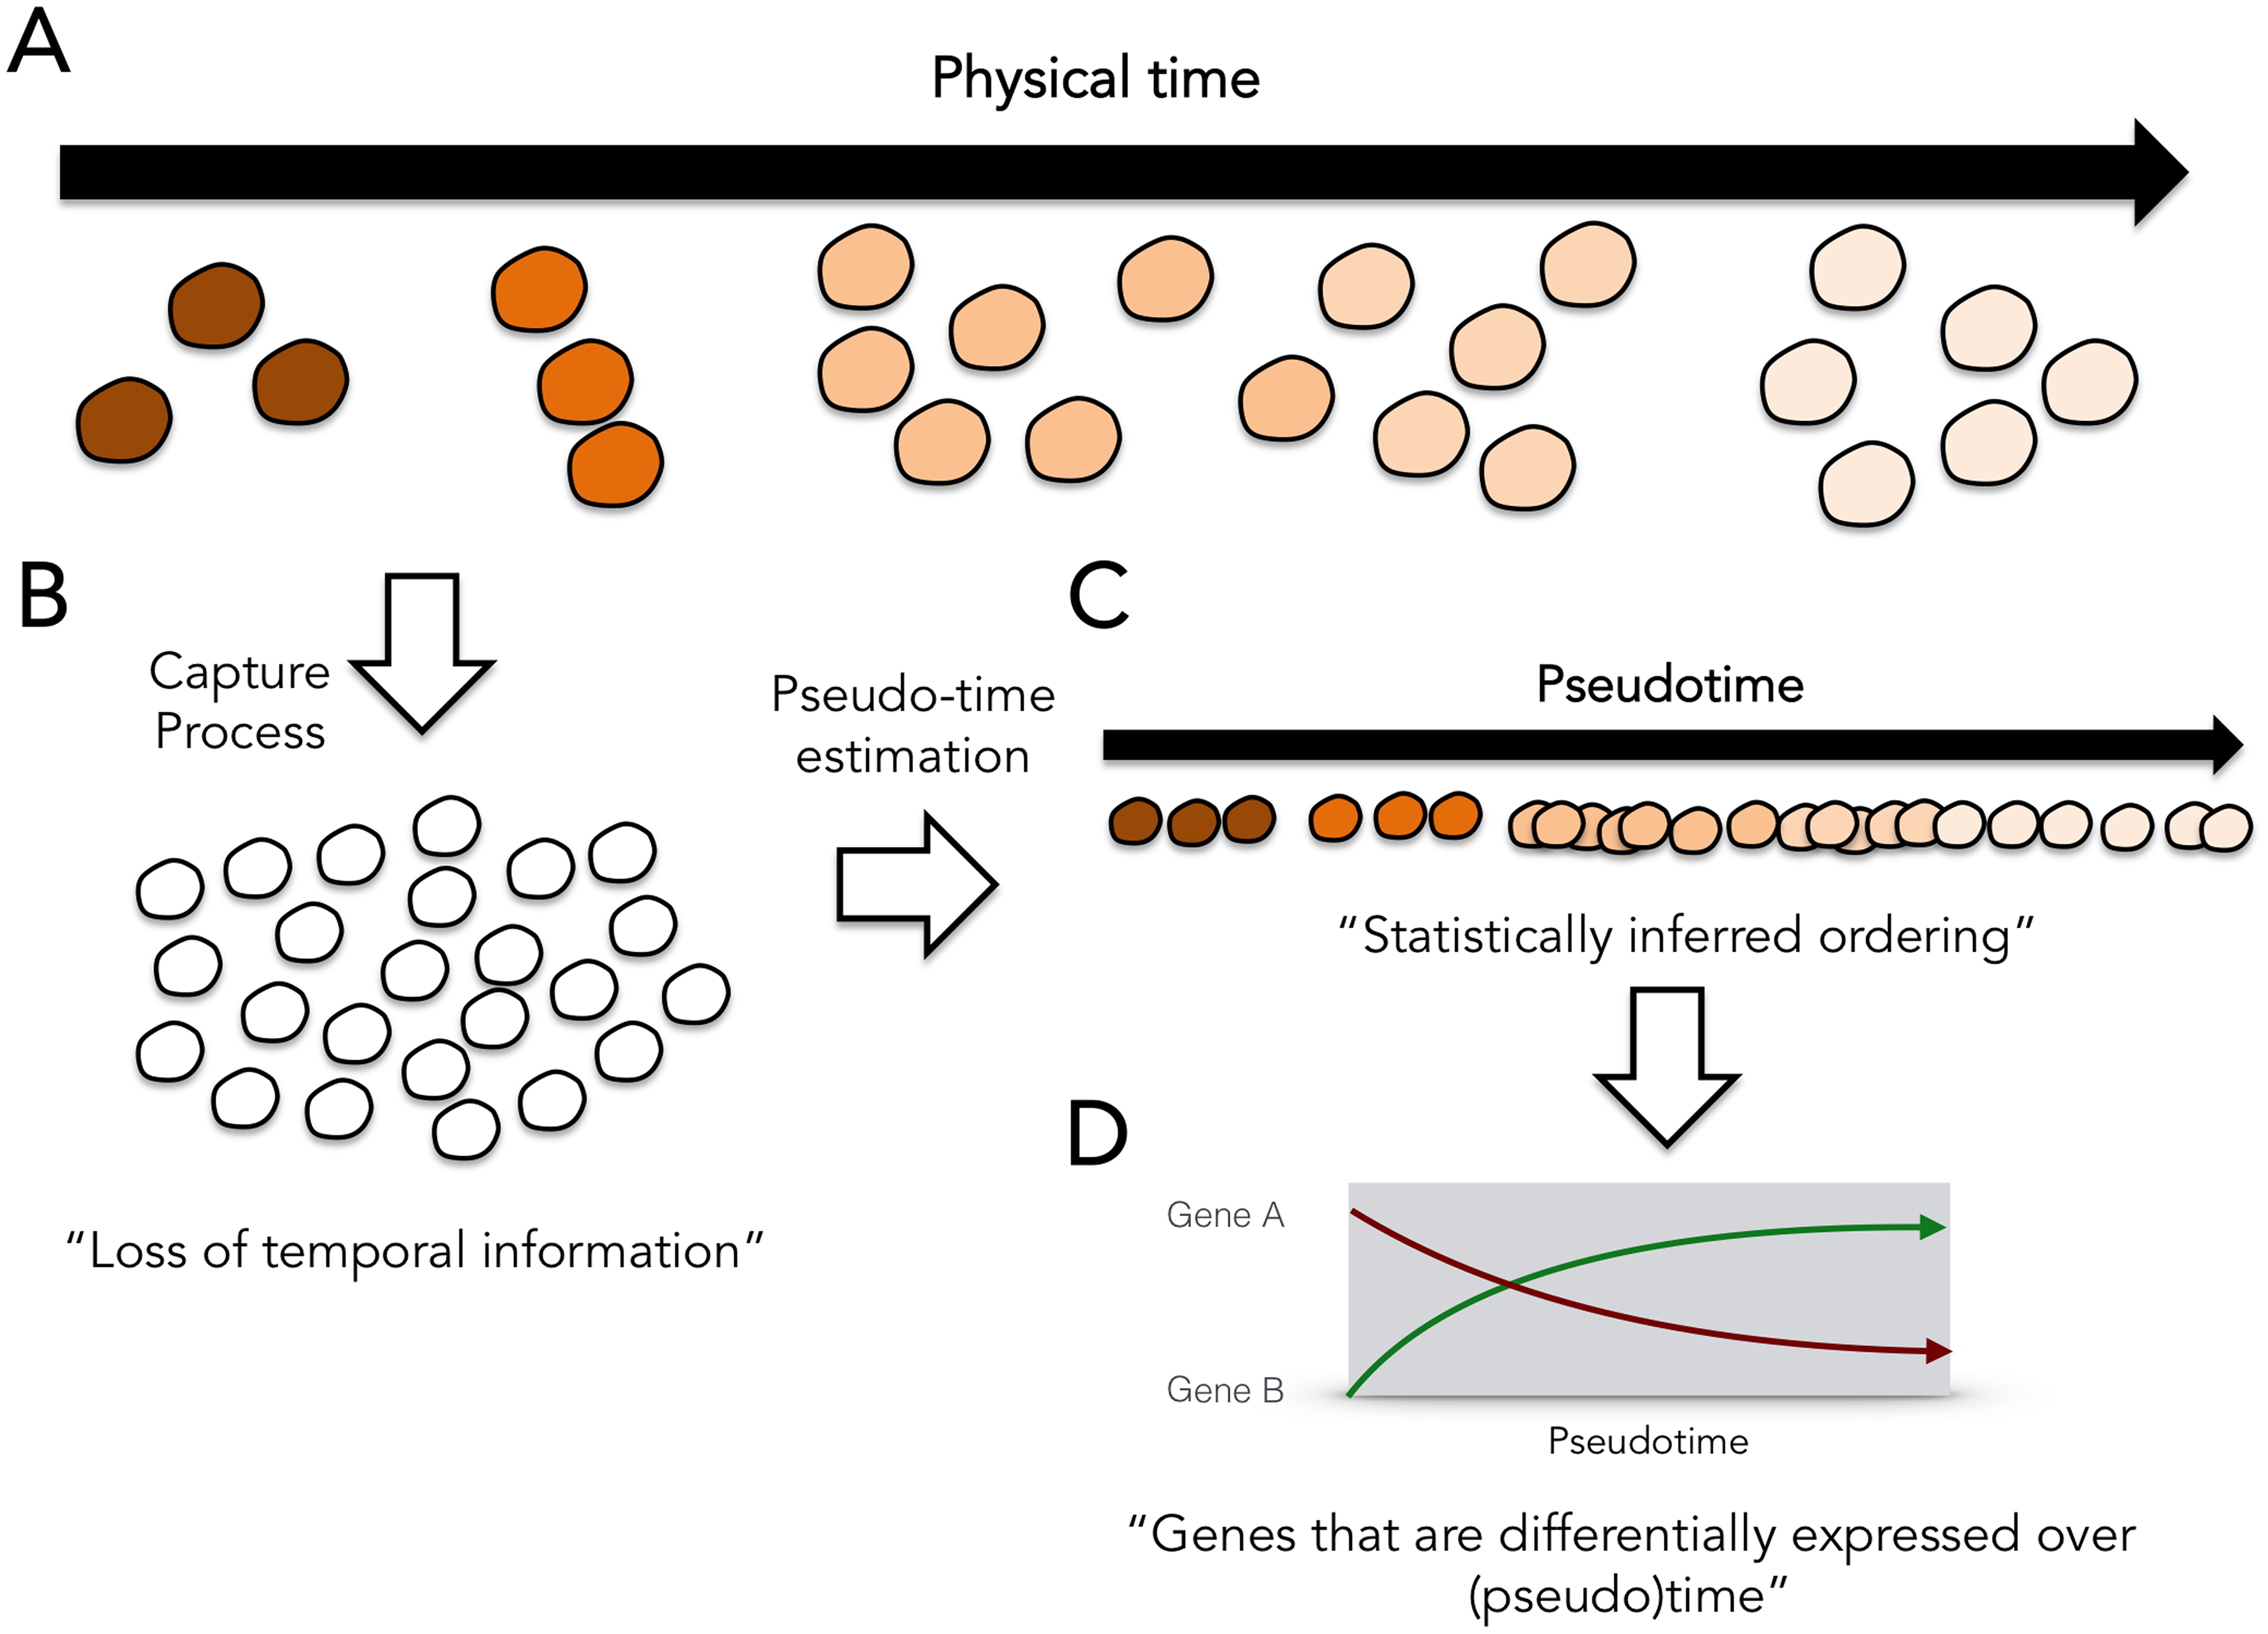
\includegraphics[scale=1.0]{images/fig1campbell.png}
\end{center}
\caption{\textbf{Overview of single-cell sample collection and developmental ordering.} (A) For a set of cells (each single cell is indicated by a circle), a true developmental time associated with its development is a latent variable (indicated by the color gradient) that accounts for a large proportion of the variance in the transcriptomic profiles. (B) While this developmental time is a true feature of these cells, current technologies do not allow for the capture of this physical/developmental time ordering (aside from rare exceptions). (C) Thus, computational and statistical approaches are required to approximate the developmental time. This approximation is referred to as \textit{pseudotime}. (D) Once ordering of cells can be approximated, genetic factors associated for a developmental process can be inferred. Image reproduced without permission from \cite{campbell2016order}. }
\end{figure}


\subsection{Unsupervised learning}

Unsupervised learning is a term used to describe the inference of hidden structure from ``unlabeled'' data. \cite{hastie2009springer} In contrast to supervised or reinforcement learning, the accuracy of the structure that is inferred by the algorithm cannot be obtained directly in unsupervised learning. Conversely, supervised learning approaches use an outcome of interest (often accuracy) to help guide feature selection and parameter approximations in model building. As the true developmental ordering ``label'' is typically absent from single cell datasets, unsupervised approaches are required for both feature (gene) selection and parameter estimation in inferring the developmental gradient from the observed feature space. \newline \newline
In classical statistics, a popular form of unsupervised learning is \textbf{method of moments} where unknown parameters are related to the moments of random variables. \cite{hastie2009springer} From values of moment-based estimators and the form of the relationship between random variables and parameters, a straightforward application of unsupervised learning leads to the estimation unknown parameters. In high-dimensional data settings, a canonical technique for unsupervised learning is \textbf{principal component analysis} (PCA), which infers a set of orthogonal dimensions that maximize the variance of the samples through a linear transformation of a feature set. \cite{jolliffe2002principal} Though PCA is adept at inferring structure that accounts for variance in observations (single cells) even with covariance in the feature set (gene expression values), its specification as a linear dimensionality reduction technique has limited its utility in situations where non-linear representations of the observed data may best achieve the learning task at hand (as has been hypothesized with cellular developmental time). \cite{cannoodt2016computational} To this end, a class of methods called \textbf{Gaussian process latent variable models} (GPLVM) have been proven useful to derive structure from high-dimensional data settings in especially in machine-learning contexts. \cite{lawrence2004gaussian} Here, I'll examine the formulation of PCA and GPLVM in a likelihood-based framework, which enables a straightforward approximation of uncertainty in this application of unsupervised learning. 


%%%%%%%%%%%%%%%%%%%%%%%%%%%%%%%%%%%%
\section{Setting}

A typical representation of single cell data is represented in a matrix $\mathbf{Y}$ of dimension $M$ genes x $N$ cells. Elements of this matrix $\mathbf{Y}$ are populated by the observed gene counts that result from a scRNA-Seq experiment. \textbf{Figure 2A} provides an example of such a matrix, which will serve as the data basis for pseudotime estimation approaches. While $M > 20,000$ in most scRNA-Seq experiments, considerable covariation is observed in the gene expression values. Like many high-dimensional settings, some smaller number $d$ ($d < M$) ``true signals'' are parameters of the data-generating mechanisms associated with the $M$ genes. In scRNA-Seq, two of thse $d$ ``signals'' or latent variables may be the  developmental ordering of the cell and the cell's stage in the cell cycle. \newline
\begin{figure}[H]
\begin{center}
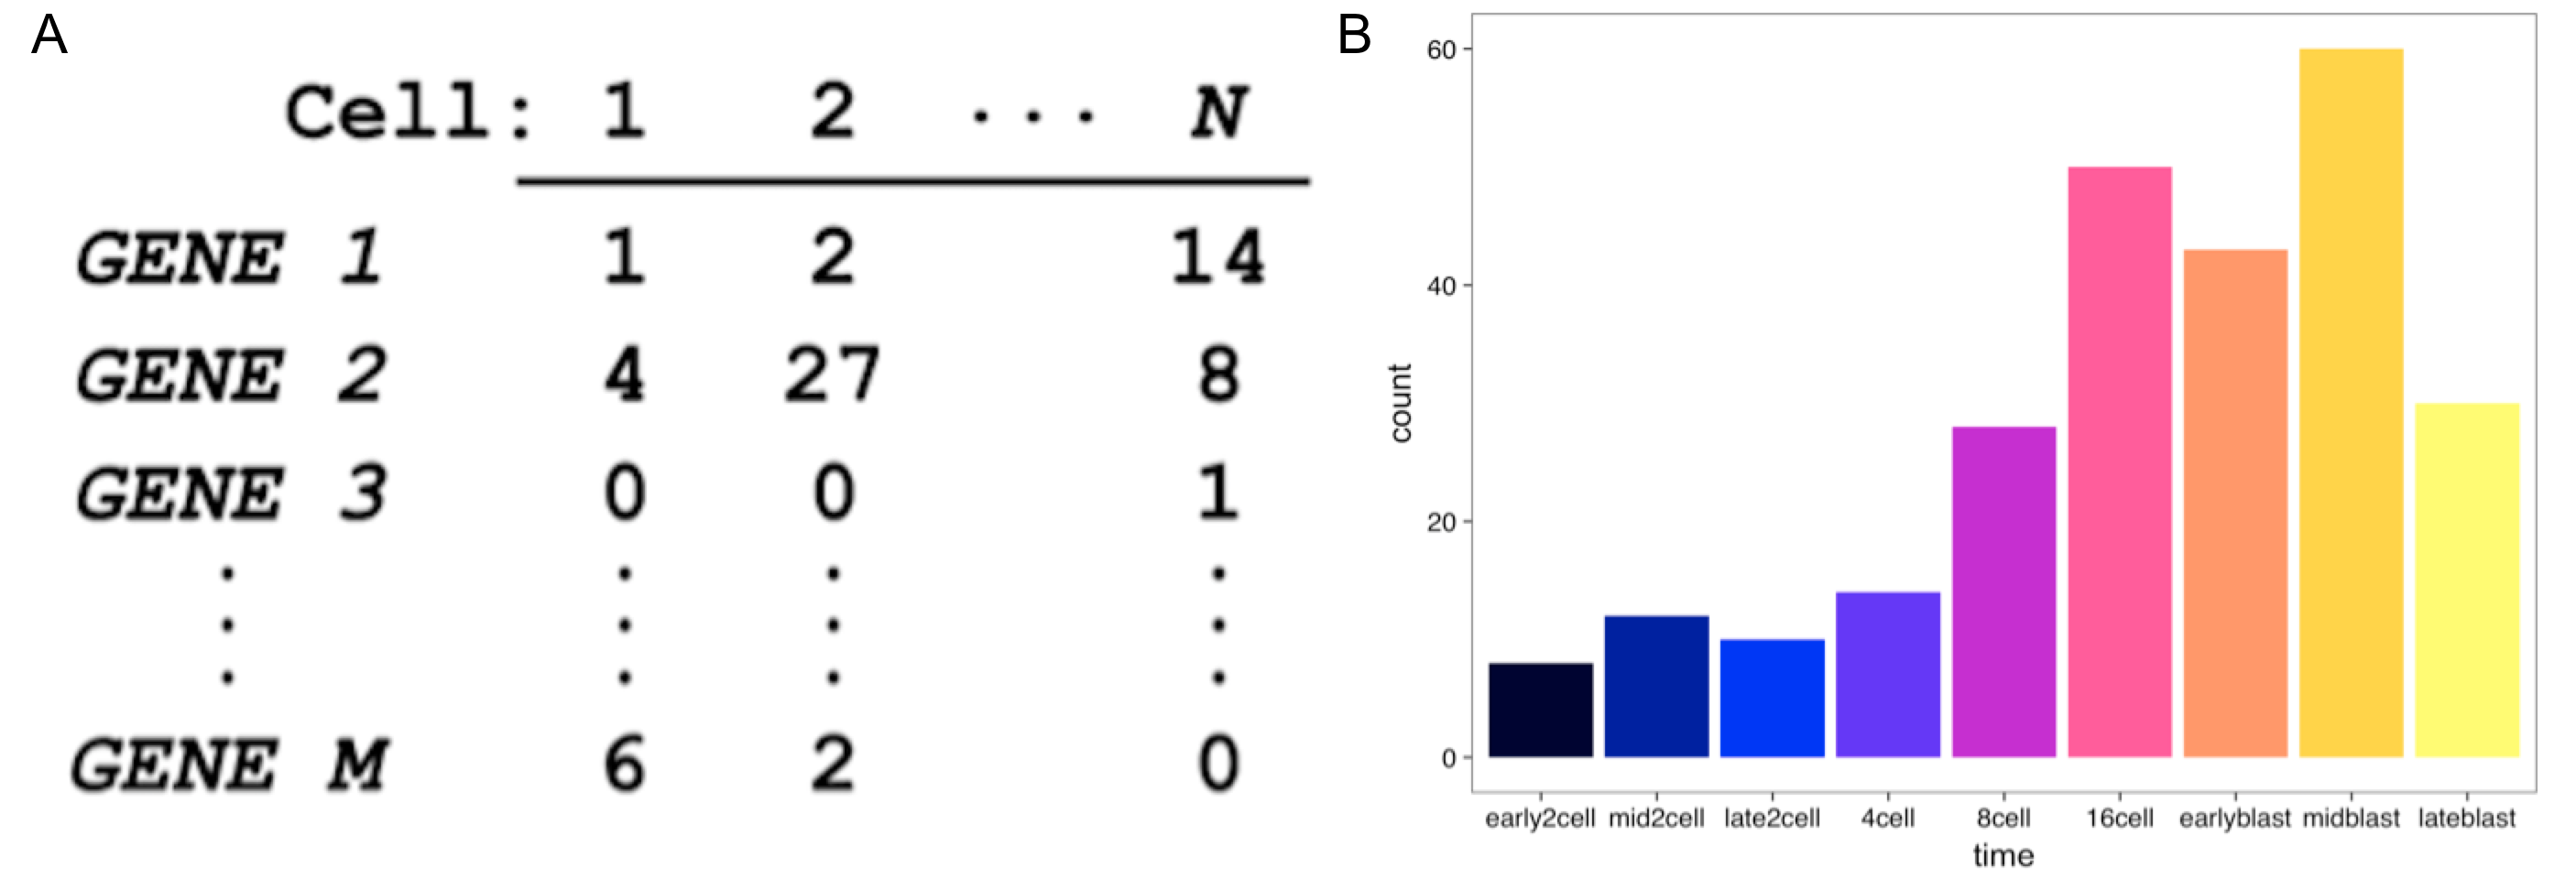
\includegraphics[scale=0.3]{images/Figure2.png}
\end{center}
\caption{\textbf{Data summary for single cell analysis setting.} (A) An example of a data matrix $\mathbf{Y}$ of dimension $M$ genes x $N$ cells. This matrix (which may be normalized by a variety of techniques) serves as the input for unsupervised learning methods discussed herein. Image reproduced without permission from \cite{macosko2015highly} (B) Annotation of the $N$ single cells used in the sample data analysis. Embryonic stem cells were derived from \textit{in vitro} fertilized mice at various stages of embryonic development and $M$ gene transcripts were quantified using the SMART-Seq2 protocol as previously described. \cite{deng2014single} The color gradient from dark to light reflects the known developmental ordering (uncommon in most scRNA-Seq experiments) and is consistent throughout the figures presented in this document. }
\end{figure}

\noindent As an example, cells cycling in G2 that are early in development may be highly expressing genes \textit{GENE 3, GENE M-4,} and \textit{ GENE M-2} and lowly expressing \textit{GENE 2} and \textit{GENE 15,000} whereas cells in G1 that are also early in development may be highly expressing \textit{GENE 3, GENE M-4,} and \textit{GENE M}. Thus, we seek to compute a matrix $\mathbf{L}$ of $d$ latent variables x $N$ cells that gives an approximation of the reduced dimensionality features responsible for the observed gene expression counts. It has been hypothesized \cite{cannoodt2016computational} and experimentally verified \cite{lonnberg2017single} that the latent variable that explains the most variance in the cells is associated with developmental time in scRNA-Seq datasets that come from a single, sufficiently dynamic biological system. Thus, we will specify a vector $P$ of dimension $1$ x $N$ that is a column vector of $\mathbf{L}$ that explains the most variance in the data to be our estimates of pseudotime for these $N$ cells. $P$ can be thought of as principal component 1 (PC1) or GPLVM1, depending on the method of unsupervised learning. Note that while the cell cycle latent variable has previously been estimated using GPLVM \cite{buettner2015computational} and may be of biological interest, this latent variable is not explicitly considered in this manuscript.  \newline\newline
Finally, to evaluate the efficacy of these unsupervised learning approaches, I will examine the the squared correlation ($r^2$) between the vector $P$ estimated by different approaches and the true developmental ordering of a set of $ > 250$ murine embryonic stem cells. \textbf{Figure 2B} shows the 9 true developmental timepoints that were availabel through a carefully controlled experiment as previously described. \cite{deng2014single} Notably, this scRNA-Seq dataset is exceptional in that these developmental annotations are available and a feature of the dataset whereas this is typically unobserved in most data settings. The true developmental ordering will be represented by an integer vector of dimension $1$ x $N$ with elements $\{ 1, 2, ..., 9\}$ ($1 = $ early2cell; $9 =$ lateblast; see x-axis of \textbf{Figure 2B}), which will be correlated with $P$. 


%%%%%%%%%%%%%%%%%%%%%%%%%%%%%%%%%%%%
\section{Methods}

Over a dozen computational approaches have been proposed to infer pseudotime from scRNA-Seq data (recently reviewed in \cite{cannoodt2016computational}) though nearly all of these methods 1) do not provide an explicit form of pseudotime inference or 2) allow for uncertainty in the resulting pseudotime estimations. 



\subsection{Principal component analysis}

PCA is a form of unsupervised learning through linear dimensionality reduction. Though many different methods have been proposed to compute the principal components of a matrix, the following approach is most common. For a matrix $\mathbf{Y}$ with dimension $M$ x $N$  (as shown in \textbf{Figure 2A}), the cell-cell covariance matrix can be computed--

$$ \mathbf{\Sigma} = E(\mathbf{Y^{T}Y}) - \mathbf{\mu^T\mu}$$
where $\mathbf{\mu} = E(\mathbf{Y})$. Next, the spectral decomposition of the covariance matrix $\mathbf{\Sigma}$ can be computed using the following form--

$$\mathbf{\Sigma} a_j = \lambda_j a_j$$
for $j \in (1, ..., N)$. Then $a_j$ represent the eigenvectors of the data matrix $\mathbf{Y}$. Note the ordering of $j$ is meaningful-- 
$$ \lambda_1 \geq \lambda_2 \geq ... \geq \lambda_N \geq 0$$

\subsection{Factor analysis}

In the 1940s and 1950s, Whittle \cite{whittle1952principal} and Young \cite{young1941maximum} provided a likelihood-based framework that enabled the derivations of principal components using a factor analysis framework. Notably, this likelihood-based framework enabled a probablistic interpretation of PCA, enabling uncertainty in both the components and the loadings to be estimated from a posterior distribution. 

$\mathbf{Y}$ is a $D$ x $n$ matrix. $\mathbf{x}$ is a $d$ x $n$ matrix ($d < D$). Want to relate $\mathbf{x}$ and $\mathbf{Y}$ and assume that the relationship is linear--

$$ \mathbf{Y = Wx} + \epsilon$$<br>
where $W$ is a $D$ x $d$ matrix. <br><br>

By convention (after locating the matrix),<br><br> $$\mathbf{x} \sim \mathcal{N} (0, \mathbf{I})$$<br>
where $\mathbf{I}$ is the identity matrix of dimension $d$ x $d$. 

\subsection{Probablistic PCA}

pPCA \cite{tipping1999probabilistic}

$\psi_i$ element of the diagonal of $\Psi$; add constraint $\psi_i = \sigma^2$<br><br>
Assume $\sigma^2$ known, MLE yields same $W$ as PCA <br><br>
$$  \mathcal{L} = \frac{-N}{2}\{ D\log(2\pi) + \log|\mathbf{C}| + \textrm{tr}(\mathbf{C}^{-1}\mathbf{\Sigma})  \}   $$<br>
$$\mathbf{C} = \mathbf{WW^T }+ \mathbf{\Psi} $$ <br>
$$  \mathbf{x} = \mathbf{C^{-1}W^{T}Y}$$

Probablistic PCA (Tipping and Bishop)
- Assuming $\sigma^2$ may not be reasonable; want to estimate it from the data (keep in likelihood)
- Can estimate $\mathbf{W}, \sigma^2$ using EM and with a prior over $\mathbf{x}$

For  $\mathbf{W_{\textrm{MLE}}}$, <br><br> $$\sigma_{MLE}^2 = \frac{1}{D-d} \sum_{j = d +1}^D \lambda_j $$

- Similarly, we can integrate over $\mathbf{W}$ given a prior, yielding <br><br>
$$  \mathbf{x} \sim  \mathcal{N} (\mathbf{C^{-1}W^{T}Y}, \sigma^2C^{-1})$$ <br>


Computational methods for inferring principal components under this likelihood framework are availabel through the \texttt{pcaMethods} \texttt{R} package.

\subsection{Bayesian PCA}
Though not utilized in this particular data analysis, the derivation of probablistic PCA enables a Bayesian framework for performing linear dimensionality reduction and putting a prior on these reduced dimensions. \cite{bishop1999bayesian} Methods for computing principal components with Bayesian priors and interpretations are also accessible through the \texttt{pcaMethods} \texttt{R} package.

\subsection{Gaussian Process Latent Variable Modeling}

\begin{equation}
\mathbf{Y} \sim  \mathcal{N} (0, \mathbf{C}), \mathbf{C} = \mathbf{WW^T }+ \mathbf{\Psi}
\end{equation}

\begin{equation}
\mathbf{C}(\mathbf{W_i},\mathbf{W_j}) = \mathbf{W_i^T}\mathbf{W_j} + \sigma^2\delta_{ij}
\end{equation}

\begin{equation}
\mathbf{C}(\mathbf{W_i},\mathbf{W_j}) = \theta_{rbf} \exp \Big(\frac{-\gamma}{2}(\mathbf{W_i}-\mathbf{W_j})^{T}(\mathbf{W_i}-\mathbf{W_j})  \Big) + ...
\end{equation}


- (2) being a special case (linear, iid) of (3)
- Computationally more challenging, but there are fast algorithms out there






%%%%%%%%%%%%%%%%%%%%%%%%%%%%%%%%%%%%
\section{Data Application}
From mice \cite{deng2014single}
A small simulation study or application to existing dataset.

\begin{figure}[H]
\begin{center}
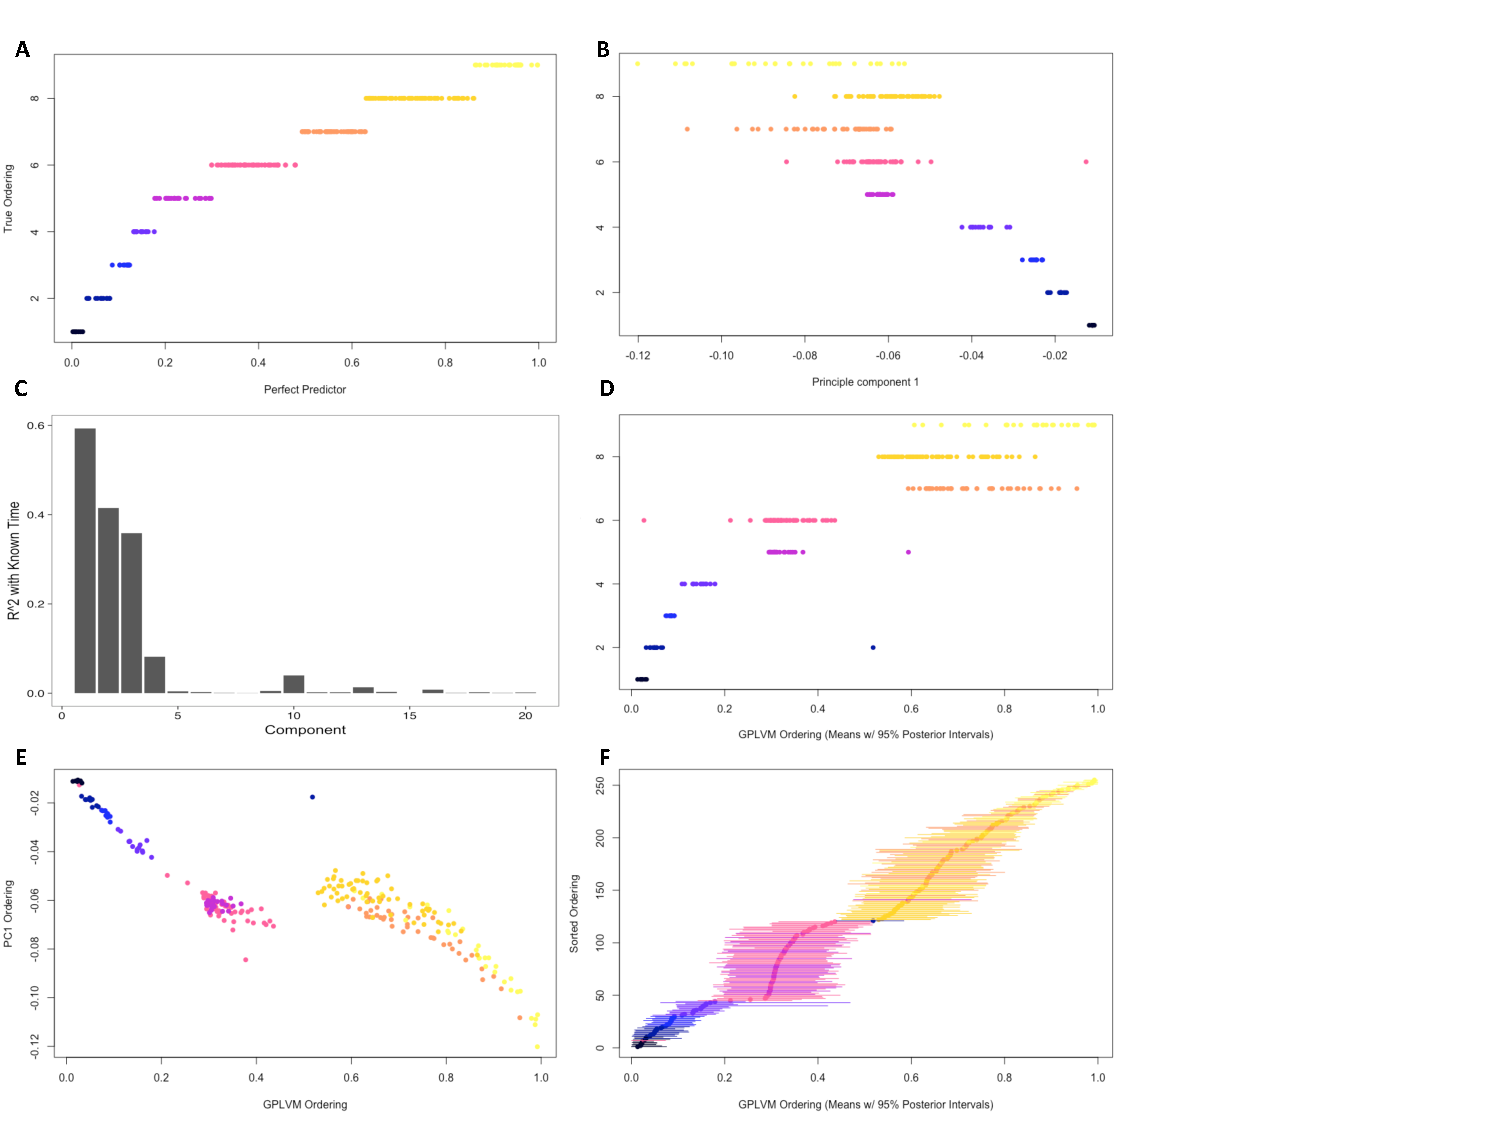
\includegraphics[scale=0.8]{images/Figure3.pdf}
\end{center}
\caption{\textbf{Summary of unsupervised learning results applied to murine embyronic stem cell development.} (A) An example of a ``perfect'' latent dimension (x-axis) where the true ordering of the nine embryonic states (y-axis) is inferred ($r^2 = 0.88$). (B) The comparison of the true developmental ordering (y-axis) against a linear unsupervised learning dimension (principal component 1), indicating a decent approximation of true developmental ordering ($r^2 = 0.59$). (C) Barplot depicting the $r^2$ for the first 20 principal components similar to what was shown for PC1 in (B). This plot suggests that a non-linear dimension reduction may best approximate the true developmental ordering. (D) The comparison of the true developmental ordering (y-axis) against a non-linear unsupervised learning dimension (Gaussian Process latent variable 1), indicating a better approximation of true developmental ordering ($r^2 = 0.78$). (E) Comparison of linear (y-axis; PC1) and non-linear (x-axis; GP latent variable 1) reduced dimensions. The non-linear unsupervised learning technique separates day 8 and day 16 development from the blastocyst samples. (F) Uncertainty associated with GP latent variable 1 depicted with the 95\% posterior confidence interval. The uncertainty computed in the posterior distribution provides a probablistic measure for pseudotime ordering of these single cell samples. }
\end{figure}


%%%%%%%%%%%%%%%%%%%%%%%%%%%%%%%%%%%%
\section{Discussion / Conclusion}

In brief, the application of GPLVM provided a good approximation of the cellular developmental time from the specificed sample of murine embryonic stem cells. Notably, the extra flexibility afforded through non-linear feature reduction lead to a better squared correlation ($r^2 = 0.78$) with the true developmental ordering than the linear dimension reduction through PCA. ($r^2 = 0.59$) Moreover, as PCA is a special case of GPLVM, \cite{lawrence2004gaussian} this approach is a flexible, encompassing approach for unsupervised learning that has gained considerable popularity in a variety of data applications outside of single-cell biology. 
\newline \newline
As previously mentioned, the utility of GPLVM in this data setting extends beyond the estimation of cellular development time but has been shown to approxmiate other latent variabels in single cell gene expression values, including the cell cycle stage. \cite{buettner2015computational} In specific biological applications, GPLVM have been applied to resolve Th1/Tfh cell-fate decisions in mice exposed to malaria, providing novel insights into the genetic perturbations associated with T-cell response and memory to foreign antigens. \cite{lonnberg2017single} More generally, Welch $et$ $al.$ showed that GPLVM provide a flexible means to infer development ordering in single cells using not just RNA profiles but also chromatin accessibility, methylation, and histone modifications derived from single-cell experiments. \cite{welch2017manifold} Thus, for unsupervised learning in single-cell biology, GPLVM provides a generalized, flexible tool for handling a variety of data types and modeling a variety of desired structures with statistical ease and confidence.  
\newline \newline
An important feature of GPLVM as shown in the \textbf{Methods} section of this document is the formal probalistic interpretation of the latent dimensions inferred from this class of unsupervised learning. As such, uncertainty in the estimates of these variables can be quantified and visualized as shown in \textbf{Figure 3F}. These uncertainty estimates are a vital component of uncovering true variation associated with dynamic  processes in developmental biology, such as cancer progression \cite{corces2016lineage} and hematopoiesis. \cite{buenrostro2017single} The application of GPLVM to our murine embryonic scRNA-Seq data suggests that resolving meaningful gene expression differences within \textit{a priori} labeled populations may not be sensible. However, differences between classes of labels (\textit{i.e.} differences in gene expression between early2cell, 8/16cell, and blastocyst) may evaluated with statistical confidence. 
\newline \newline
As the richness and depth of large datasets become more prevalent in the 21st century (\textit{e.g.} transcript profiles of $> 35$ trillion cells), sophisticated statistical theory and methodologies must be developed to extract meaningful structure from these data. While carefully considered and motivated through an application to single-cell biology, methods of unsupervised learning have become a key component of many data analysis tasks for a large variety of data types. The form of pPCA and GPLVM provides a facile integration into well-established likelihood-based methods for high-dimensional data settings, making these techniques a worthwhile addition to the biostatistician's toolkit.


\section*{Accessibility}

All code and data used to generate the figures, slides, and writeup are made publicly available at \url{https://github.com/caleblareau/BST245_Final}. An \texttt{R} package for running GPLVM (tailored to single-cell data) is distributed through \texttt{Github} and can be installed typing the following command into an \texttt{R} console: \url{devtools::install_github("kieranrcampbell/pseudogp")}.  The \texttt{pcaMethods R} package for running PCA, Bayesian PCA, and Probablistic PCA is distributed via \texttt{Bioconductor} and is available at \url{http://bioconductor.org/packages/release/bioc/html/pcaMethods.html}.

\newpage{}


%%%%%%%%%%%%%%%%%%%%%%%%%%%%%%%%%%%%
\bibliographystyle{ieeetr}
\bibliography{Lareau245Final}{}

\end{document}
